
\documentclass[acmlarge,nonacm=true]{acmart}
\usepackage{adjustbox}
\usepackage{multirow}
\usepackage{graphicx}
\usepackage{afterpage}
\usepackage{subcaption}

\newcommand\blankpage{%
	\null
	\thispagestyle{empty}%
	\addtocounter{page}{-1}%
	\newpage}

%%
%% \BibTeX command to typeset BibTeX logo in the docs
\AtBeginDocument{%
  \providecommand\BibTeX{{%
    \normalfont B\kern-0.5em{\scshape i\kern-0.25em b}\kern-0.8em\TeX}}}


\begin{document}
	
	\begin{titlepage}
		\begin{center}
			\vspace*{1cm}
			
\includegraphics[width=0.7\textwidth]{fig/ntu_logo}
			\vspace{0.8cm}
			\linebreak
			\Huge
			\textbf{Experiment 1: Parametric Curves}
			
			\vspace{0.5cm}
			\LARGE
			CZ2003 Computer Graphics and Visualization
			
			\vspace{1.5cm}
			\textbf{SS3}\\
			
			\begin{table}[h]
				\begin{tabular}{lc}
					Name & Matric Number \\\hline
					Pang Yu Shao & U17216\underline{\textbf{80}}D \\
				\end{tabular}
			\end{table}
			
			
			
			\vfill
			
			\vspace{0.8cm}
			
			
			
			\Large
			SCHOOL OF COMPUTER SCIENCE AND ENGINEERING\\
			NANYANG TECHNOLOGICAL UNIVERSITY\\
			SINGAPORE\\
			2nd Febraury 2021
			
		\end{center}
	\end{titlepage}

 

%%
%% The "title" command has an optional parameter,
%% allowing the author to define a "short title" to be used in page headers.
\title{CZ2003 Computer Graphics and Visualization}

%%
%% The "author" command and its associated commands are used to define
%% the authors and their affiliations.
%% Of note is the shared affiliation of the first two authors, and the
%% "authornote" and "authornotemark" commands
%% used to denote shared contribution to the research.


\author{Pang Yu Shao}
\email{C170134@e.ntu.edu.sg}
\affiliation{\institution{Nanyang Technological University}}

%%
%% By default, the full list of authors will be used in the page
%% headers. Often, this list is too long, and will overlap
%% other information printed in the page headers. This command allows
%% the author to define a more concise list
%% of authors' names for this purpose.
\renewcommand{\shortauthors}{Pang Yu Shao}






%%
%% This command processes the author and affiliation and title
%% information and builds the first part of the formatted document.

% \begin{teaserfigure}
% 	\includegraphics[width=\textwidth]{bccell}
% 	\caption{Breast Cancer Cell. Photograph by National Cancer Institute [Public domain], via Wikimedia
% 		Commons. (\url{https://w.wiki/kS3}).}
% 	\Description{A breast cancer cell seen through an electron microscope.}
% \end{teaserfigure}
% \maketitle



\tableofcontents
\newpage
\section{Defining Surfaces Parametrically}
\subsection{Plane Passing Through Three Defined Points}
To define the plane parametrically, we can use the following formula: \(P = P1+u(P2-P1)+v(P3-P1)\)\\
Therefore, with the 3 points \((N, M, 0),\ (0, M, N),\ (N, 0, M)\), we get:\\
\(x(u,v) = N - Nu = \mathbf{8 - 8u}\)\\
\(y(u,v) = M + Mv = \mathbf{10 + 10v}\)\\
\(z(u,v) = Nu + Mv = \mathbf{8u + 10v}\)\\
\(\mathbf{u,v \in [0,1]}\)

\begin{figure}[H]
	\begin{subfigure}{.33\textwidth}
	  \centering
	  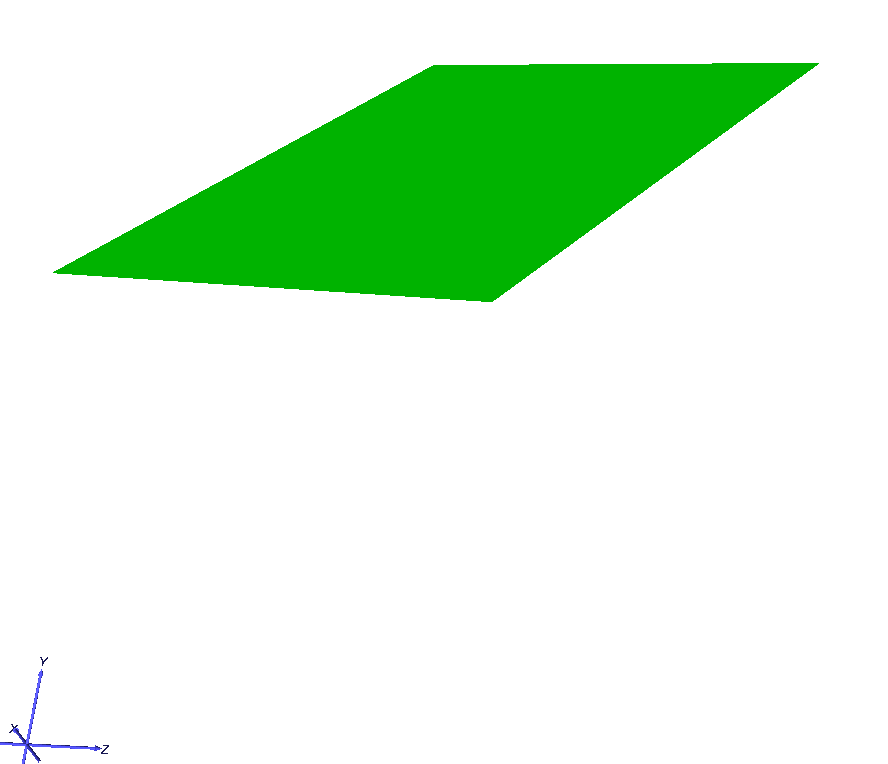
\includegraphics[width=.8\linewidth]{fig/1a1_1}
	  \caption{Resolution: 1 1}
	\end{subfigure}%
	\begin{subfigure}{.33\textwidth}
	  \centering
	  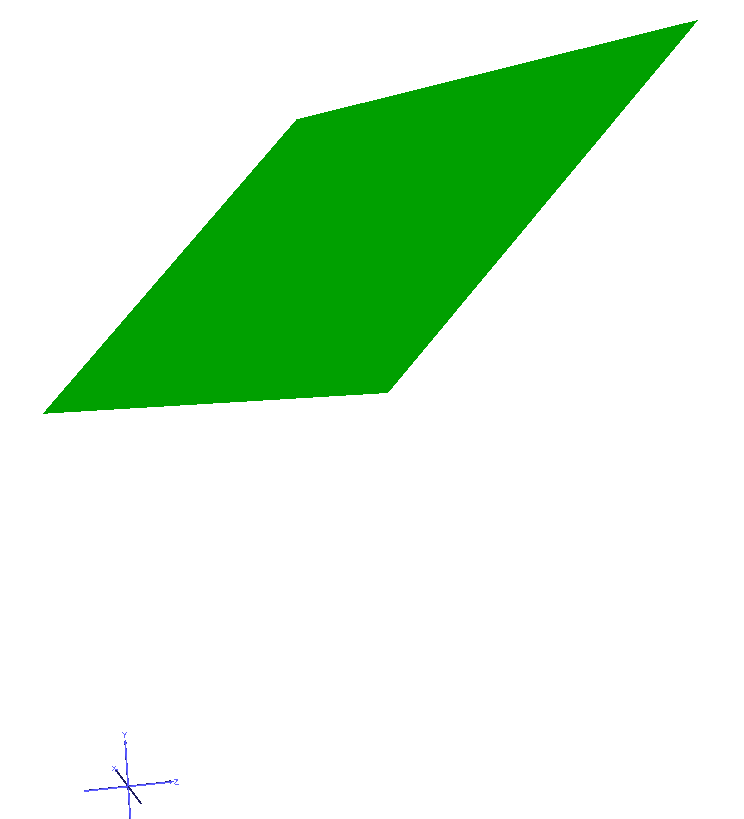
\includegraphics[width=.8\linewidth]{fig/1a10_10}
	  \caption{Resolution: 10 10}
	\end{subfigure}
	\begin{subfigure}{.33\textwidth}
		\centering
		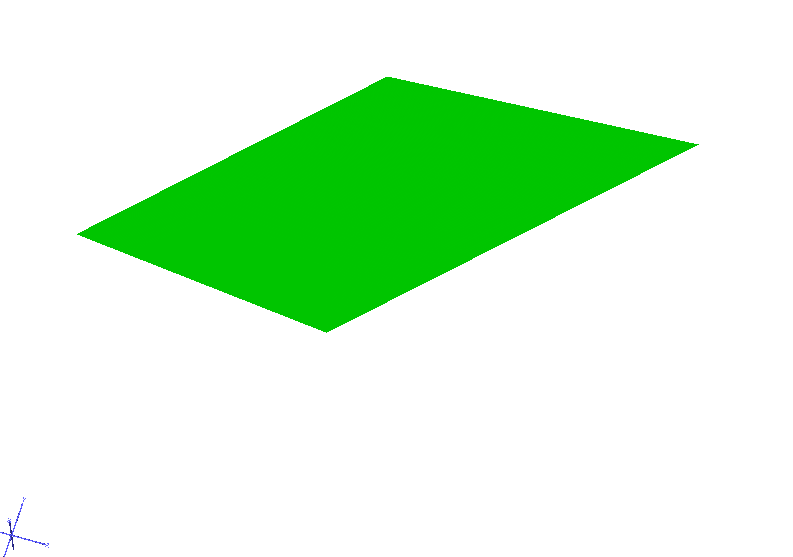
\includegraphics[width=.8\linewidth]{fig/1a1000_1000}
		\caption{Resolution: 1000 1000}
	  \end{subfigure}
	\caption{Plots of the plane defined in "\textbf{1a.wrl}" with differing resolutions}
	\label{fig:1a}
\end{figure}
As seen in Fig. \ref{fig:1a} above, a sampling resolution of \textbf{1} for both u and v is 
sufficient for drawing the plane as it has no curvature and having a higher resolution would
produce the exact same drawing.

\subsection{Triangular Polygon with Three Defined Vertices}
To define the Triangular Polygon, we use the formula for defining Bilinear Surface Parametrically,
and we set two of the points to be the same point, essentially resulting in a Triangular polygon.\\\\
\(P = P1 + u(P2-P1) + v(P3-P1+u(P4-P3-(P2-P1)))\)\\
Let P4 = P3, we get:\\
\(P = P1 + u(P2 - P1) + v(P3 - P1) + uv(P1 - P2)\)\\
Therefore, with the 3 points \((N, M, 0),\ (0, M, N),\ (N, 0, M)\), we get:\\
\(x(u,v) = N - Nu + Nuv = \mathbf{8 - 8u + 8uv}\)\\
\(y(u,v) = M - Mv = \mathbf{10 - 10v}\)\\
\(z(u,v) = Nu + Mv - Nuv = \mathbf{8u + 10v - 8uv}\)\\
\(\mathbf{u,v \in [0,1]}\)

\begin{figure}[H]
	\begin{subfigure}{.33\textwidth}
	  \centering
	  
\includegraphics[width=.8\linewidth]{fig/1b1_1}
	  \caption{Resolution: 1 1}
	\end{subfigure}%
	\begin{subfigure}{.33\textwidth}
	  \centering
	  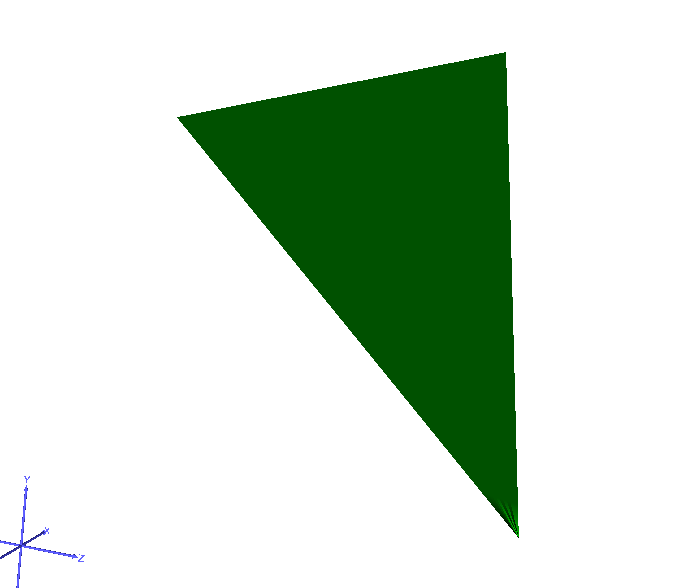
\includegraphics[width=.8\linewidth]{fig/1b10_10}
	  \caption{Resolution: 10 10}
	\end{subfigure}
	\begin{subfigure}{.33\textwidth}
		\centering
		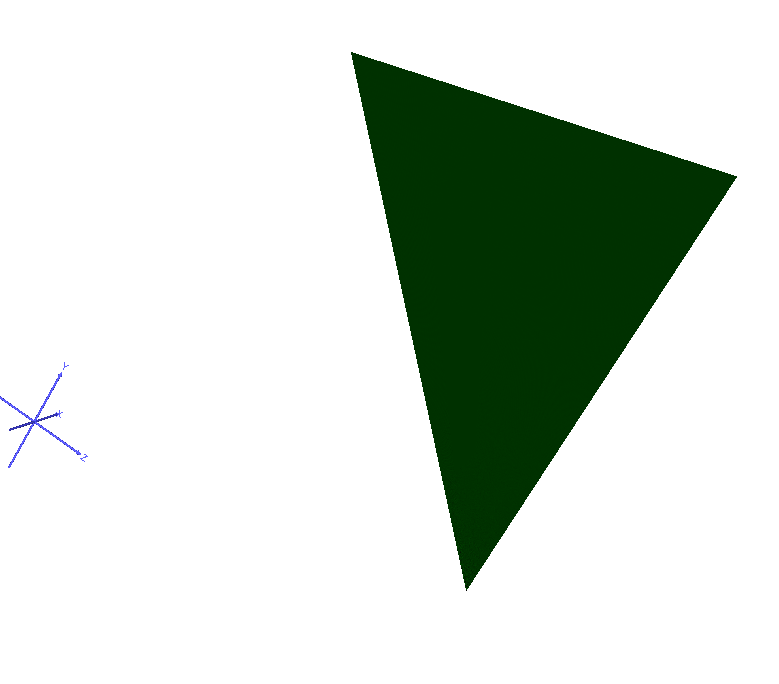
\includegraphics[width=.8\linewidth]{fig/1b1000_1000}
		\caption{Resolution: 1000 1000}
	  \end{subfigure}
	\caption{Plots of the Triangular Polygon defined in "\textbf{1b.wrl}" with differing resolutions}
	\label{fig:1b}
\end{figure}

As seen in Fig. \ref{fig:1b} above, a sampling resolution of \textbf{1} for both u and v is 
sufficient for drawing the triangular polygon as it has no curvature and having a higher resolution would
produce the exact same drawing.


\subsection{Origin-Centered Ellipsold with Defined Semi-axes}
An elipsoid can be parametrically defined using the following functions:\\
\(x = acos(u)sin(v)\)\\
\(y = bsin(u)\)\\
\(z = ccos(u)cos(v)\)\\
Where \(u \in [-\pi/2, \pi/2]\) and \(v \in [-\pi, \pi]\). Therefore, we can get:\\
\(x = Ncos(-\pi/2 + \pi u)sin(-\pi + 2\pi v) = \mathbf{8cos(-\pi/2 + \pi u)sin(-\pi + 2\pi v)}\)\\
\(y = Msin(-\pi/2 + \pi u) = \mathbf{10sin(-\pi/2 + \pi u)}\)\\
\(z = (N+M/2)cos(-\pi/2 + \pi u)cos(-\pi + 2\pi v) = \mathbf{9cos(-\pi/2 + \pi u)cos(-\pi + 2\pi v)}\)\\
\(u,v \in [0,1]\)

\begin{figure}[H]
	\begin{subfigure}{.33\textwidth}
	  \centering
	  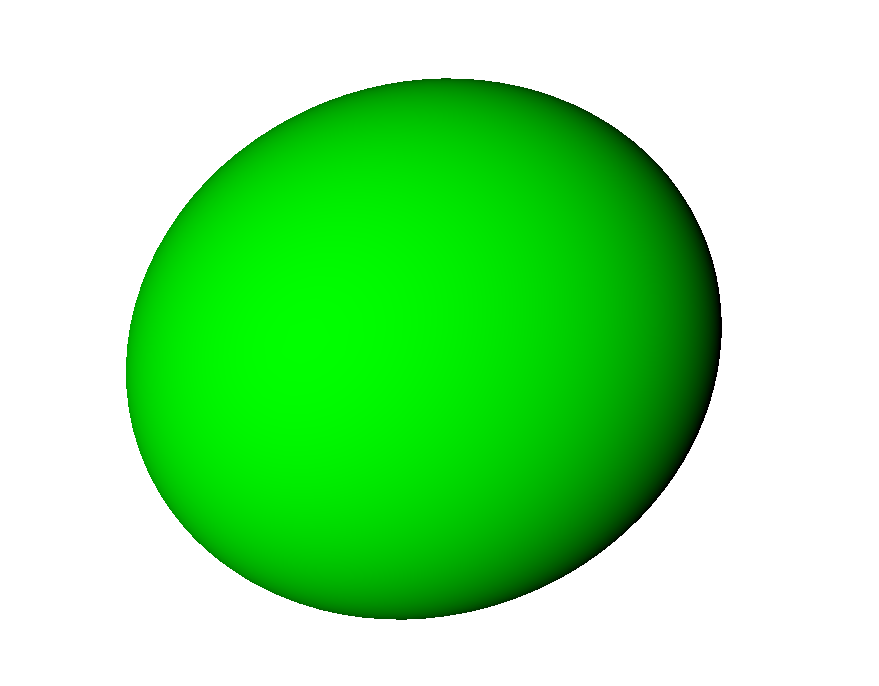
\includegraphics[width=.8\linewidth]{fig/1c50_100}
	  \caption{Resolution: 50 100}
	\end{subfigure}%
	\begin{subfigure}{.33\textwidth}
	  \centering
	  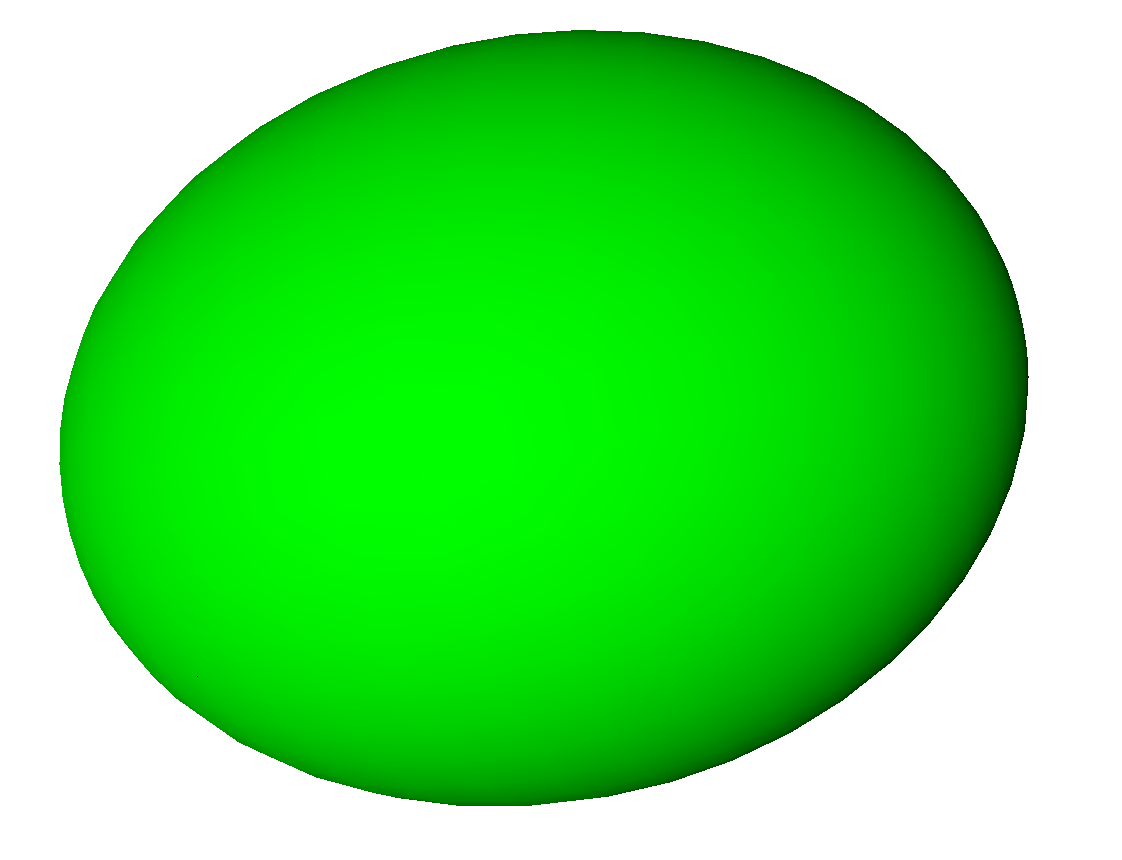
\includegraphics[width=.8\linewidth]{fig/1c25_50}
	  \caption{Resolution: 25 50}
	\end{subfigure}
	\begin{subfigure}{.33\textwidth}
		\centering
		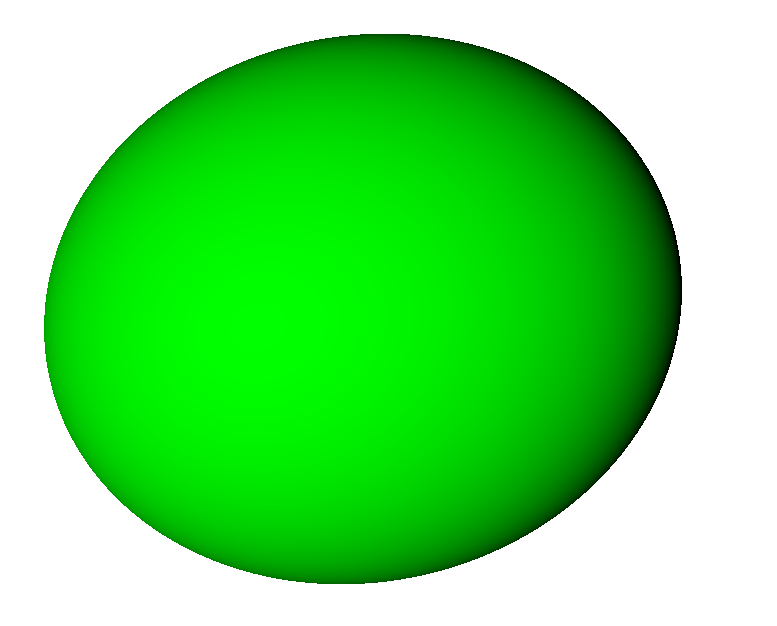
\includegraphics[width=.8\linewidth]{fig/1c100_200}
		\caption{Resolution: 100 200}
	  \end{subfigure}
	\caption{Plots of the Triangular Polygon defined in "\textbf{1c.wrl}" with differing resolutions}
	\label{fig:1c}
\end{figure}

The sampling resolution for v is chosen to be 2 times larger than that of u as the coefficient of v is 
2 times larger. As seen in Fig. \ref{fig:1c} above, the best resolution obtained was 50, 100 for u and v respectively.
By decreasing the resolution to 25 and 50, the interpolations could be seen when zoomed in. When the resolution was increased
instead to 100 and 200, no visible difference could be seen.

\bibliographystyle{ACM-Reference-Format}
\newpage






\end{document}
\endinput
%%
%% End of file `sample-acmlarge.tex'.
